\chapter{Разъём и схемы подключения}
Семиконтактный разъём KF2510 пронумерован на плате. Ориентируйтесь по фотографии и номерам, а не только по цветам проводов. Контакт 1: K30/KL30, питание; 2: V2; 3: V1; 4: 1WRE, One-Wire; 5: KL, зарезервированная K-Line; 6: выход +5 В, не более 30 мА; 7: GND, масса.

На схеме вольтметра указаны зарезервированная K-Line и ограничение тока выхода +5 В. Общие допустимые напряжения аналоговых входов не приведены. Указание 12 В для Check Engine не означает, что другие входы допускают такое напряжение. Используйте схему для конкретного датчика.

В оригинальных иллюстрациях сохранены английские подписи; соответствующие функции объяснены в тексте руководства.

\begin{figure}[H]
\centering
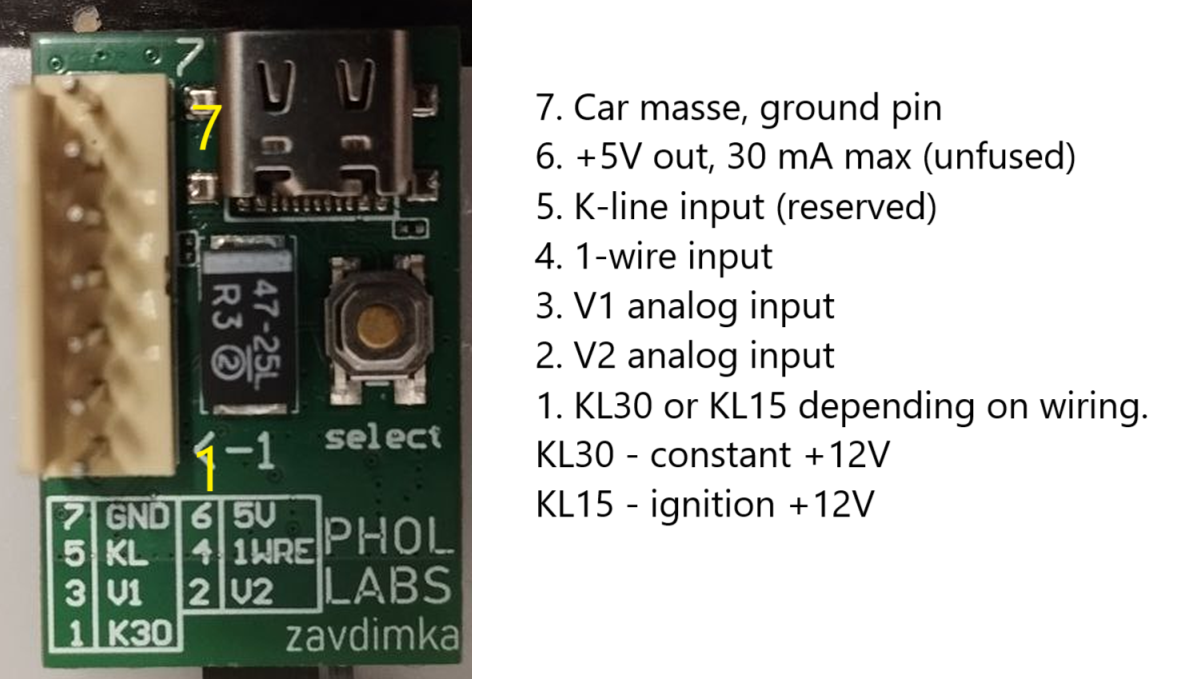
\includegraphics[width=.85\textwidth,height=.60\textheight,keepaspectratio]{figures/ivevo/image20.png}
\caption{Разъём и схемы подключения}
\end{figure}
\clearpage
\section{Вольтметр}

\begin{figure}[H]
\centering
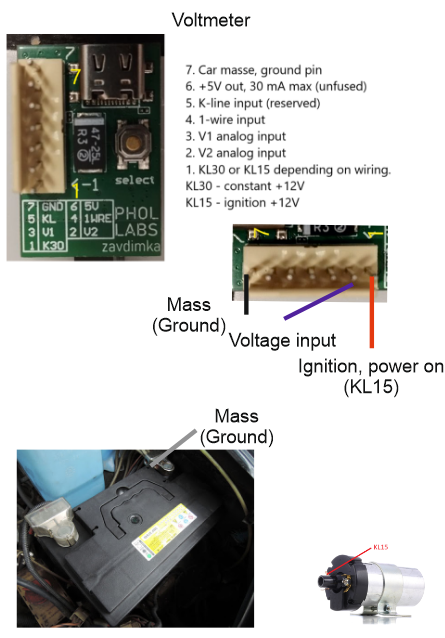
\includegraphics[width=.85\textwidth,height=.60\textheight,keepaspectratio]{figures/ivevo/image5.png}
\caption{Вольтметр}
\end{figure}
\clearpage
\section{Индикатор передачи}

\begin{figure}[H]
\centering
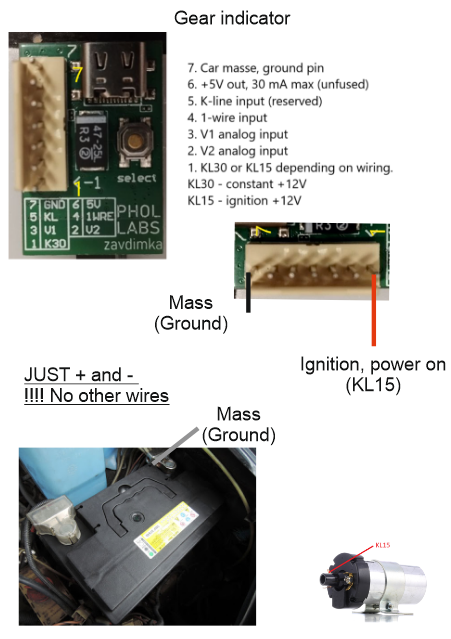
\includegraphics[width=.85\textwidth,height=.60\textheight,keepaspectratio]{figures/ivevo/image6.png}
\caption{Индикатор передачи}
\end{figure}
\clearpage
\section{Давление масла}

\begin{figure}[H]
\centering
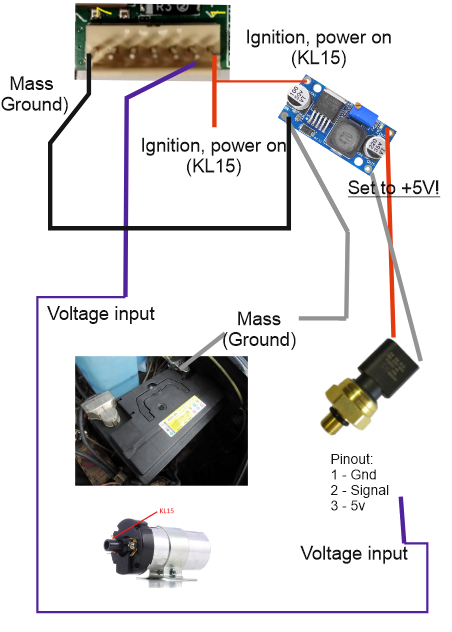
\includegraphics[width=.85\textwidth,height=.60\textheight,keepaspectratio]{figures/ivevo/image1.png}
\caption{Давление масла}
\end{figure}
\clearpage
\section{Термометр NTC}

\begin{figure}[H]
\centering
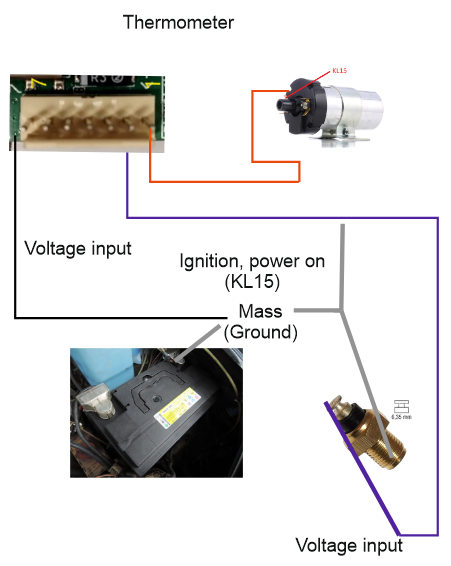
\includegraphics[width=.85\textwidth,height=.60\textheight,keepaspectratio]{figures/ivevo/image13.png}
\caption{Термометр NTC}
\end{figure}
\clearpage
\section{Цифровой термометр}

\begin{figure}[H]
\centering
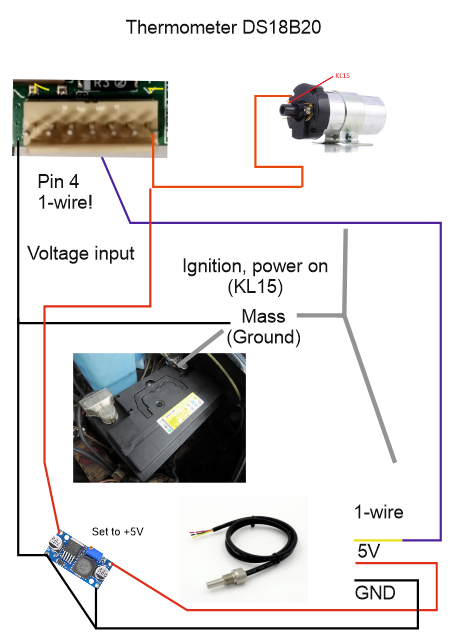
\includegraphics[width=.85\textwidth,height=.60\textheight,keepaspectratio]{figures/ivevo/image8.png}
\caption{Цифровой термометр}
\end{figure}
\clearpage
\section{Широкополосная лямбда}

\begin{figure}[H]
\centering
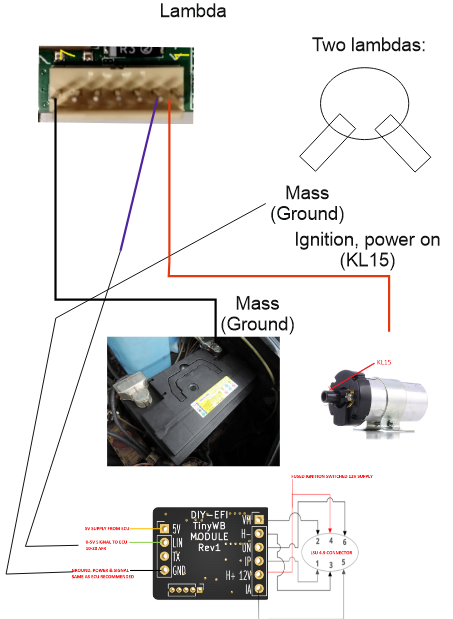
\includegraphics[width=.85\textwidth,height=.60\textheight,keepaspectratio]{figures/ivevo/image3.png}
\caption{Широкополосная лямбда}
\end{figure}
\clearpage
\section{Наддув}

\begin{figure}[H]
\centering
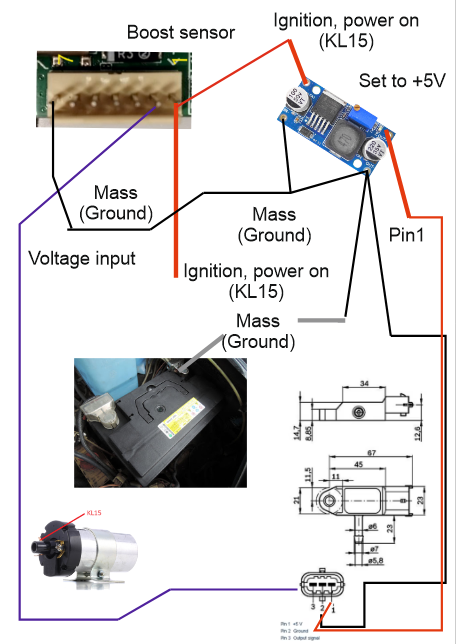
\includegraphics[width=.85\textwidth,height=.60\textheight,keepaspectratio]{figures/ivevo/image17.png}
\caption{Наддув}
\end{figure}
